\documentclass{article}

\usepackage{color}
\usepackage{graphicx}
\usepackage{tabulary}

\usepackage{enumitem}
\usepackage{caption}

\usepackage{xeCJK}
\setCJKmainfont{AR PL UKai CN}
\usepackage{listings}

\title{\begin{huge}
算法设计文档
\end{huge}}  
\author{wuziheng}

\begin{document}
\maketitle
\paragraph{结合质量报告对整个工程的流程分析,我们可以理清整个工程分为采集,算法,显示三个步骤,当然比赛项目的框架设计是侧重算法的,其他部分都简化处理,调用了Opencv的函数。如果是实际工程,在整个流水线上还可以做更好的优化,例如将ISP与采集分开,DMA直接搬运到算法buffer等等,这些是笔者在其他项目中的经验之谈。这里,我们将对整个算法的设计做一些简要的介绍。}

\section{算法流程分析}
\paragraph{算法主要流程图如下Figure.1,算法包含四组关键的全局变量,他们负责记录对于输入图像产生各个阶段的结果}

	\begin{itemize}[leftmargin=*]
	\item[]Proposals: 维护当前帧检测出的目标区域框的位置和Label信息(直到下一帧的Proposals生成)
	\item[]BadProposals: 维护当前程序记录的标记不会出现手势的区域和Label信息,例如恒定不动的人脸区域,长期出现FalsePostive的区域等等。
	\item[]Total: 标准的命名应该为RectResultWithoutLabel,记录当前帧Viola-Jones分类器检测的cv::Rect结果。
	\item[]TotalA: 标准的命名应该为RectResultWithLabel,根据Total更新的当前帧确认检出的的cv::Rect与其分类的Label信息。
	\end{itemize}
	
	\begin{figure}[htb]
	\centering
	\centerline{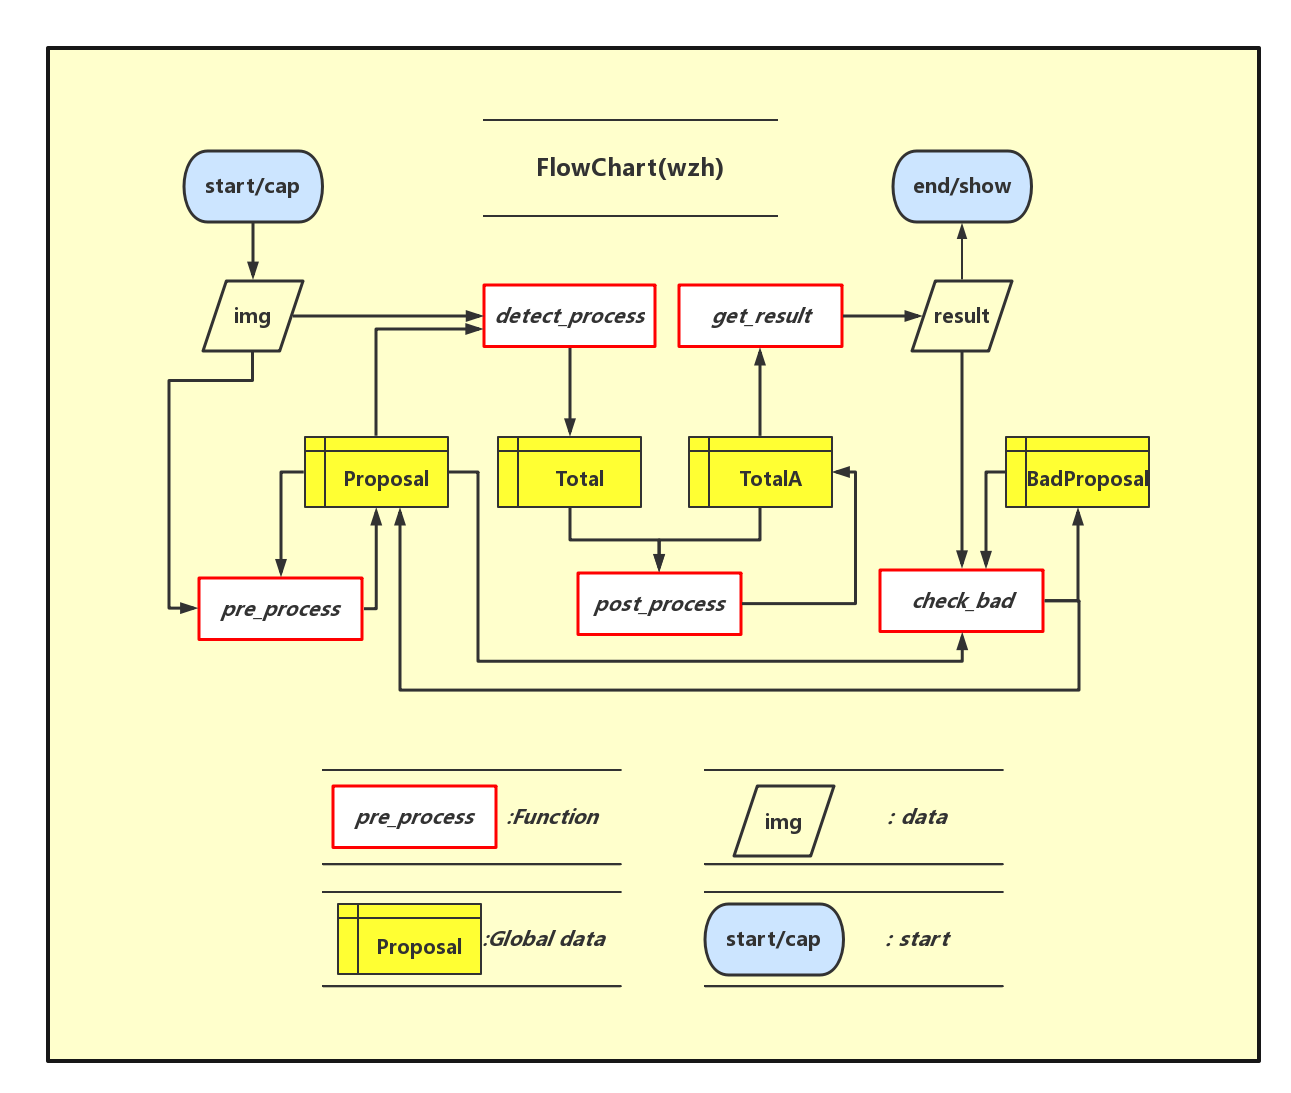
\includegraphics[scale=0.3]{pic/flow.png}}
	\caption{算法流程图}
	\label{fig:label}
	\end{figure}

\paragraph{}流程图中我们以采集为算法循环的开始,显示为一帧算法循环的结束。每一帧算法循环都在根据输入图像更新上述四组全局变量。这里的流程图是算法中main\_frame的检测流程图,实际上在比赛版本的算法中还有一个sub\_frame的检测流程。两者唯一的区别就在与sub\_frame直接使用TotalA的结果为基础来更新Proposals,而不在做预处理。接下来我们将逐一分析流程中的处理函数。

\section{处理函数简介}
	
\paragraph{\emph{pre\_process}:} 预处理输入图像,肤色检测定位,结合上一帧Proposals生成检测分类的区域Proposals。对于480p的输入图像可以在1.8到2.1ms之间完成,具体检测效果可以见详细分析与配图。
\paragraph{\emph{detect\_process}:} 根据Proposals的标记信息选择合适的搜索顺序,完成手势的定位&分类检出,输出结果到Total。这里结合了视频信息中的同一手势的连续性的特征。按照标记顺序进入特定的搜索顺序在五个手势的检出中能够将平均2.5次的分类器搜索时间降低到1.2次左右,如果需求更多手势的检出,这里的提速比更大。
\paragraph{\emph{post\_process}:} 比对Total与TotalA,通过连续性分析消除偶然出现的误检测,并对检出框进行连续性记录。这里平均一帧图像消耗10us以内的时间可以消除掉大部分临时出现的误检,大大降低了框架对Viola-jones分类器的precision的需求,使得训练过程中能够更倾向于去训练高recall的分类器模型,增加了框架的鲁棒性与实用性。
\paragraph{\emph{get\_result}:} 标准输出环节,根据TotalA中对检出框连续性的记录与预设的阈值生成最终的检出结果,并根据use\_cnn的选项选择是否再送入后端的cnn进行再确认。
\paragraph{\emph{check\_bad}:}: 通过\emph{get\_result}输出的结果比对Proposals从而生成BadProposals,并标记,更新相应的Proposals标志位。这里,可以利用长期出现在Proposals中却不产出任何手势这一信息标记并去除掉\emph{get\_result} 检测出的人脸区域,大大节省了\emph{detect\_process}的时间,因为该函数时间是随Proposals总面积线性增加的。

\section{函数实现与结果分析}
	\subsection{\emph{pre\_process}}对于输入的原始图像,我们会对其做预处理,快速获取候选检测框和相应的标记。其大致包含以下几个步骤:肤色检测,连通域处理,区域标记。
\lstset{language=C++}
\begin{lstlisting}
using resq = std::pair<int,cv::Rect>
void pre_process(const cv::Mat& img, cv::Mat& res, 
std::vector<resq>& proposal, const std::vector<resq>& 
_Proposals,int scale)
\end{lstlisting}

\paragraph{{\large 肤色检测:}}将传入的img图像转换到yuv色域,通过对肤色阈值进行检测,逐点保留肤色区域。效果图见如下Figure2(这里可以采用多线程加速,但是笔者简单的处理方法是将图像resize到原图大小的1/4,而且调用的是cv::NEAREST方式,将原本需要20ms的函数缩减到1.2ms)
	\begin{figure}[htb]
	\centering
	\centerline{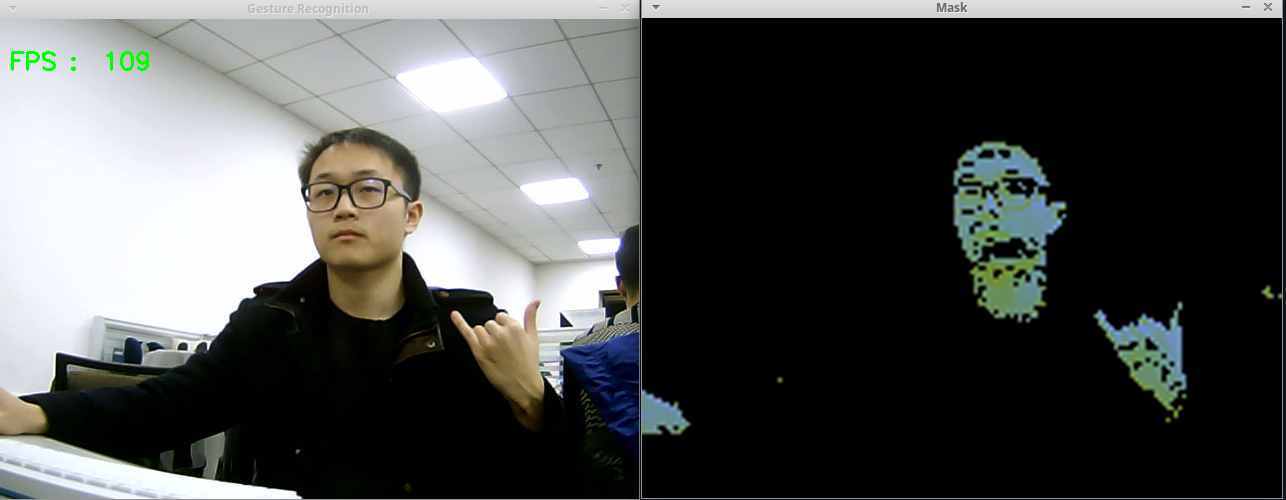
\includegraphics[width = 01.0\textwidth]{pic/handwithoutbb.png}}
	\caption{肤色检测效果}
	\label{fig:label}
	\end{figure}
	
\paragraph{{\large 连通域处理:}}在肤色检测后的图像上进行膨胀操作,弥合连通域。通过连通域轮廓搜索的方法,确定符合我们检测大小(minsize,maxsize)的连通域,获得其bounding\_box并排除掉较小的误检。效果可见配图。
	\begin{figure}[htb]
	\centering
	\centerline{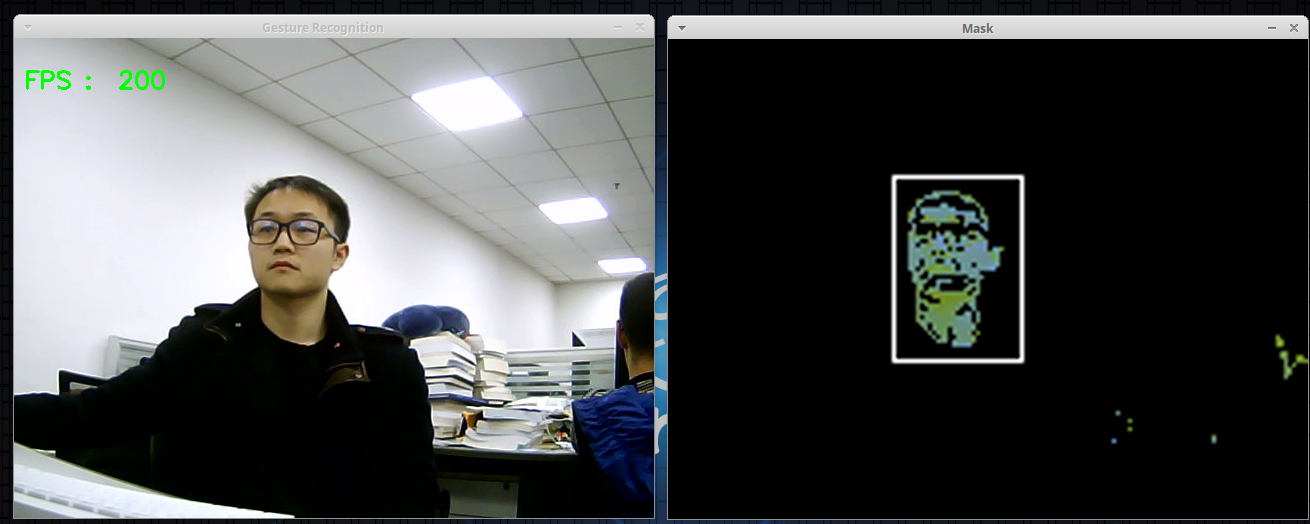
\includegraphics[width = 01.0\textwidth]{pic/facewithbb.png}}
	\caption{连通域定位效果}
	\label{fig:label}
	\end{figure}
	
\paragraph{{\large 区域标记:}}通过对比roi\_cal(lib/util.so)检测,与之前保存的Proposals进行比对,如果roi超过预设的阈值,自动获得该Proposal的标注,0到4表示的是五个手势,大于25则表示该区域已经被标记为BadProposals.
	\begin{figure}[htb]
	\centering
	\centerline{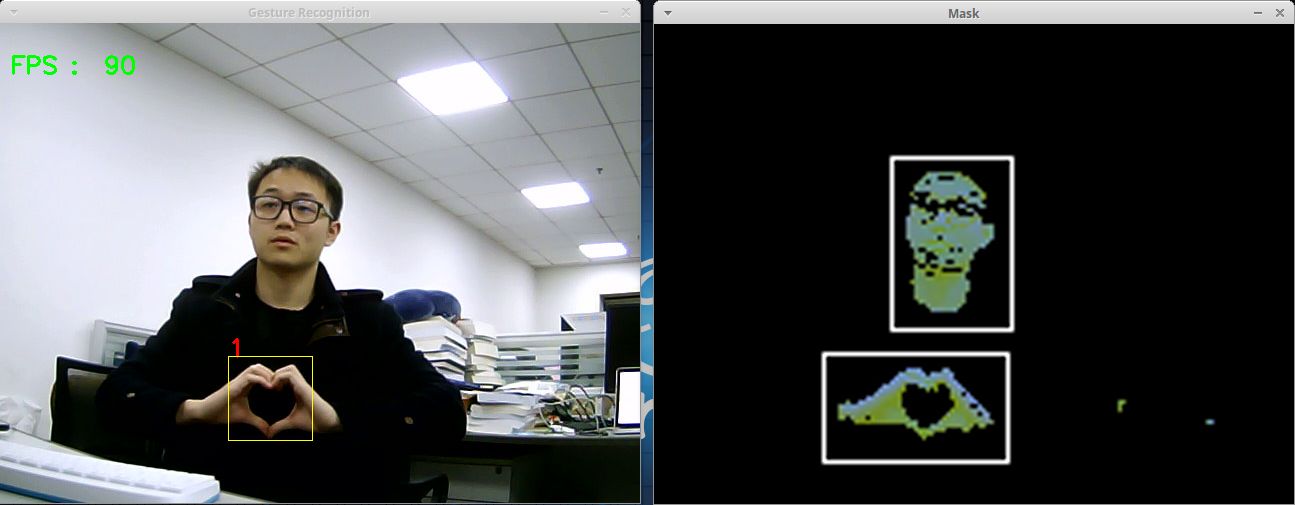
\includegraphics[width = 01.0\textwidth]{pic/faceandhand.png}}
	\caption{区域标记效果}
	\label{fig:label}
	\end{figure}
\paragraph{{\large 返回信息}} res接口保留,用于调试,实际整个函数并不修改输入img,也不返回新的图像,整个函数只负责更新Proposals.

	\subsection{\emph{detect\_process}}对于输入的每一个Proposal,我们会送入SafeEnlarge(lib/util.so)获得一个稍大一些的搜索框,然后在img上截取roi。并根据Proposal的标记送入detect\_vj函数,返回检测到的输出框和对应的手势标号。核心的加速思想是动态调整搜索顺序。

\lstset{language=C++}
\begin{lstlisting}
using resq = std::pair<int,cv::Rect>
int detect_vj(const cv::Mat& img, resq& proposal, 
std::vector<cv::Rect>& tmp, int bad_label_max);
\end{lstlisting}

\paragraph{{\large 动态调整搜索}} 关于Viola-jones分类器的特性,笔者在训练部分已经阐述过。这里我们将详细阐述动态调整搜索顺序这一思路的来源并给出相应的结果与提升。
\begin{itemize}[leftmargin=*]
\item[1]这里我们的比赛需求是5个手势的动态检出,我们训练了五个分类器,在实际操作中,对于每送入一个标记框,我们会把这个框的图像遍历五个分类器得到正确的分类结果。在这样的情况下,每一个框都的搜索时间都是五个分类器之和。
\item[2] 如果我们{\color{red}假设每一个框只含有一种手势,如果哪一个分类器检出到手势后就直接跳出循环}这样我们便可以将期望时间降低到2.5个手势分类器。但这种情况下检测时间将变的不够稳定,对于排在循环前的手势会快速检出,后面的手势则速度较慢。据此设想如果可以把会检出的手势动态调整到循环前列,必然可以提速并稳定时间。
\item[3]进一步如果我们能够在获得框的同时大致推断其最有可能出现的手势,根据这个手势来动态调整循环中的顺序,那么循环就有可能在头两个分类器就检出并跳出循环, 实际中,在高fps的情况下,我们可以假设人们变换手势的频率远远低于fps,{\color{red}所以绝大多数的情况中,期望的手势都是上一帧的手势,这也是我们\emph{pre\_process}标记手势框的核心假设}。
\end{itemize}
实际上这里笔者已经没有早期没有动态调整的版本截图了,但实际效果显示,进行动态调整后能够在完全不影响检出结果的情况下将\emph{detect\_vj}这一部分从10ms量级降低到2~4ms量级。如果需求的手势更多,这一算法的优势也将更加明显。当然,能够进行动态搜索顺序调整的前提是要给出Proposals,如果没有Proposals,我们也就无法假设全局只含有一种手势。


	\subsection{\emph{post\_process \& check\_bad}}{post\_process和check\_bad主要是完成后处理,包括对不连续误检测的消除已经对长期不检出手势的Proposal的标定。其中post\_process只是对代码块的打包并未封装成函数。下面我们会阐述两者的设计思路和实现。
\lstset{language=C++}
\begin{lstlisting}
void post_process()
void check_bad(std::vector<resq>& Proposals,
	const std::vector<resq>& CatchProposal, 
	std::vector<resq>& BadProposals)
\end{lstlisting}
\paragraph{{\large \textbf{\emph{post\_process:}}}}这一段主要是消除误检测,实际我们训练出来的viola-jones某些手势的分类器对于单帧图像而言,在recall与precision的trade-off中会发现,如果想要达到可以接受的recall,真实的precision是远远不够的。(补充一下,viola-jones可以说是标准的机器学习算法,pre-recall的trade-off自然也就很好理解了:对于部分手势,特征不够强,数据量不够大,不够大的原因一部分也是因为受到算力的制约。导致了这样的trade-off有些时候是无法避免的)所以权衡之后我们选择在单帧图像的测评中保证recall,然后利用视频流进行误检测的消除。{\color{red}\emph{post\_process}的核心假设在于如果是真实的手势,其检出在时间序列与空间坐标上应该是存在连续性的}。这里我们用iou\_cal(lib/util.so)来保证同一框在时间序列上的认证,然后标记其连续性。再次确认结果。
\paragraph{{\large \textbf{\emph{check\_bad:}}}}check\_bad是针对Proposals的操作,在Figure.3与Figure.4中我们可以清楚的看到,人脸也是会被\emph{pre\_process}标记出来的,而且相对于手势的搜索框,人脸更大,而且无可避免。如果能够准确的识别出一个候选框是否为人脸(或者其他非手势的肤色区域),我们就可以节省掉至少一半的搜索时间。{\color{red}所以check\_bad的假设就是如果一个Proposal框长期无法产生手势检出,我们就将其标记为BadProposals}.当然为了防止将区域锁死,算法将对BadProposals的更新非常敏感。
\paragraph{}实际上上面两部分算法对整个框架的稳定性(\emph{post\_process})与速度(\emph{check\_bad})至关重要。缺一不可。前者消除大部分误检测,后者提速比百分之50以上。看Figure.3与Figure.4我们可以明显发现Figure.3已经标注去掉了对人脸框的搜索,所以fps高达200.

\section{后记}
\paragraph{}实际上,上面大部分对算法框架的改进都来源于某一些假设,而这些假设都是笔者在对特定工程进行实验测试,思考算法瓶颈的时候胡思乱想来的。很多都是拍脑袋的想法,并不具有很强的推广性。笔者手快,一般有一个点子当天就敲进去改了,碰巧大部分都行之有效。所以说总结起来还是:程序员还是要少说多写,多试验。
\paragraph{}整个工程大概耗费了一个月时间,期间包括:搭建环境2天;准备数据,训练测试挑选出所有的模型,拖拖拉拉耗费了两周;改进框架,测试算法大概2周。剩下的日子就是磨磨蹭蹭的写文档,吹牛皮,期间也再次熟悉了大部分独立开发的工具Makefile,github,markdown.算是收获良多。
\paragraph{感谢:}感谢葱神(王晓葱)以及聚聚(杨颢)在整个项目过程中对我的不间断的帮助,尤其是葱神,对嵌入式的视频处理框架以及c++上的造诣,给了我很大的帮助和指导。
\end{document}